\chapter{Application description}\label{chapter:appdescription}

\section{Architecture}
The application will be developed using the Android Studio IDE.
The application will be developed using the Java programming language.
The application will use the Google ARCore framework\cite{ARCore}.
The application will use the Firebase cloud database to store the models. The application will use the QR code reader to import the models.
The application will use the Google Vision API to recognize the QR code.
As shown in Figure \ref{fig:architecture}, the architecture of the application consists of...

\begin{figure}[ht]
    \centering
    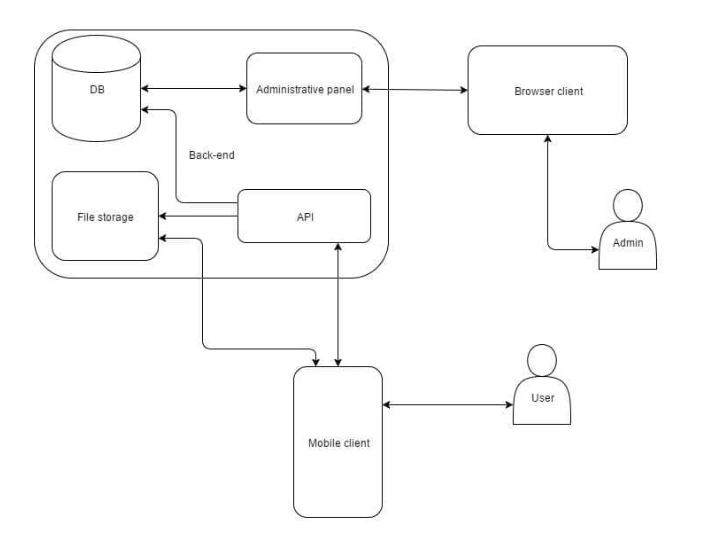
\includegraphics[width=1\textwidth]{img/architecture.png}
    \caption{Architecture}
    \label{fig:architecture}
\end{figure}

\begin{itemize}
    \item \textbf{Android Version 7.0+} - to use the application on the phone
    \item \textbf{Android Studio} - IDE for Android development
    \item \textbf{Firebase} - Cloud DataBase for where the models will be retrieved
    \item \textbf{Java} - Programming language
    \item \textbf{Google ARCore} - AR framework
\end{itemize}

\clearpage

\section{Diagrams}
\subsection*{Class diagram}

\begin{figure}[ht]
    \centering
    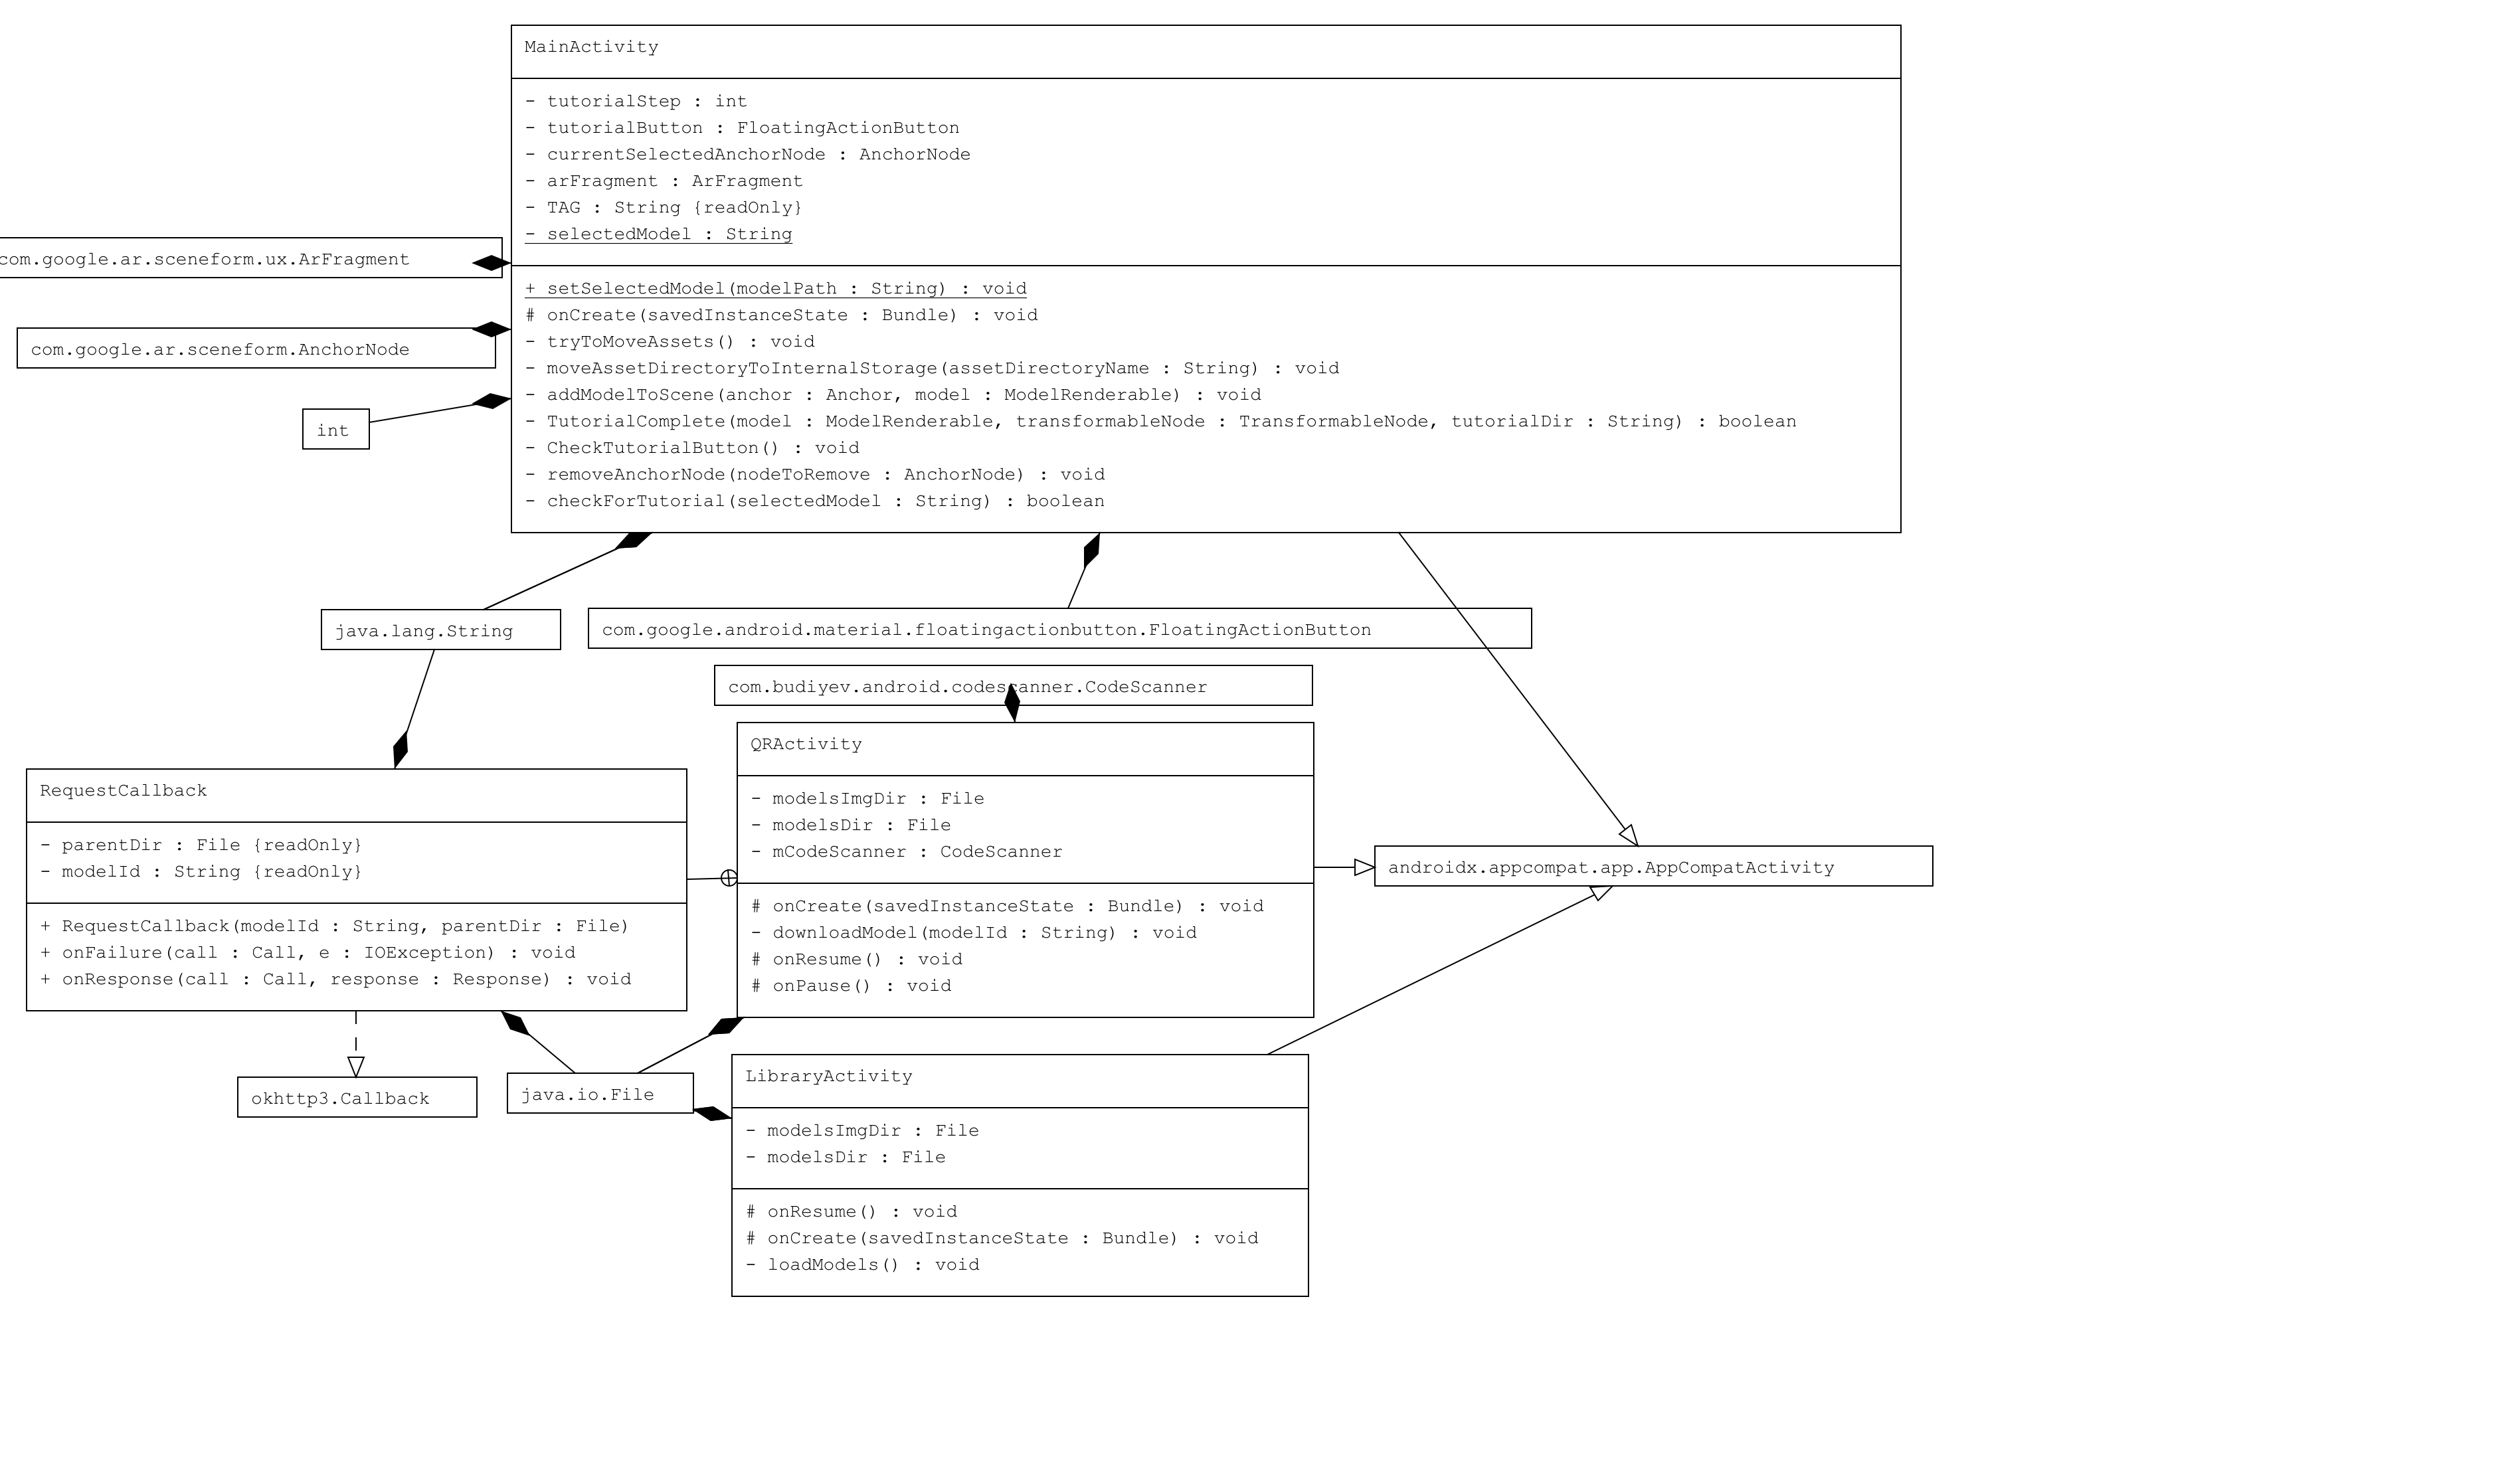
\includegraphics[width=1\textwidth]{img/ClassDiagram.png}
    \caption{Class diagram}
    \label{fig:ClassDiagram}
\end{figure}


\subsection*{Use cases}
Each user that has a smartphone capable of running the AR modules should be able to use the app. If the user has models already imported, he/she can use the app without any connection to the internet. If the user wants to import a new model, he/she will need to have an internet connection. The user will be able to import a model using the QR code. The user will be able to see the model in AR mode. The user will be able to see the guide of the model. The user will be able to see the list of all the models that he/she has imported. The user will be able to delete a model from the list of models.

\begin{figure}[ht]
    \centering
    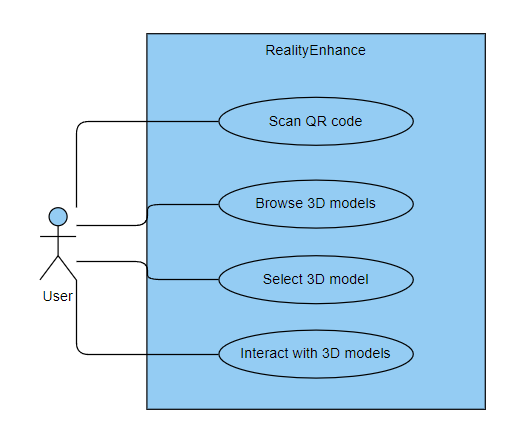
\includegraphics{img/UseCaseDiagram.png}
    \caption{Initial use case}
    \label{fig:InitialUseCase}
\end{figure}

\clearpage

\subsection*{Sequence diagram}
The user will be able to import a model using the QR code. The user will be able to see the model in AR mode. The user will be able to see the guide of the model. The user will be able to see the list of all the models that he/she has imported. The user will be able to delete a model from the list of models.

\begin{figure}[ht]
    \centering
    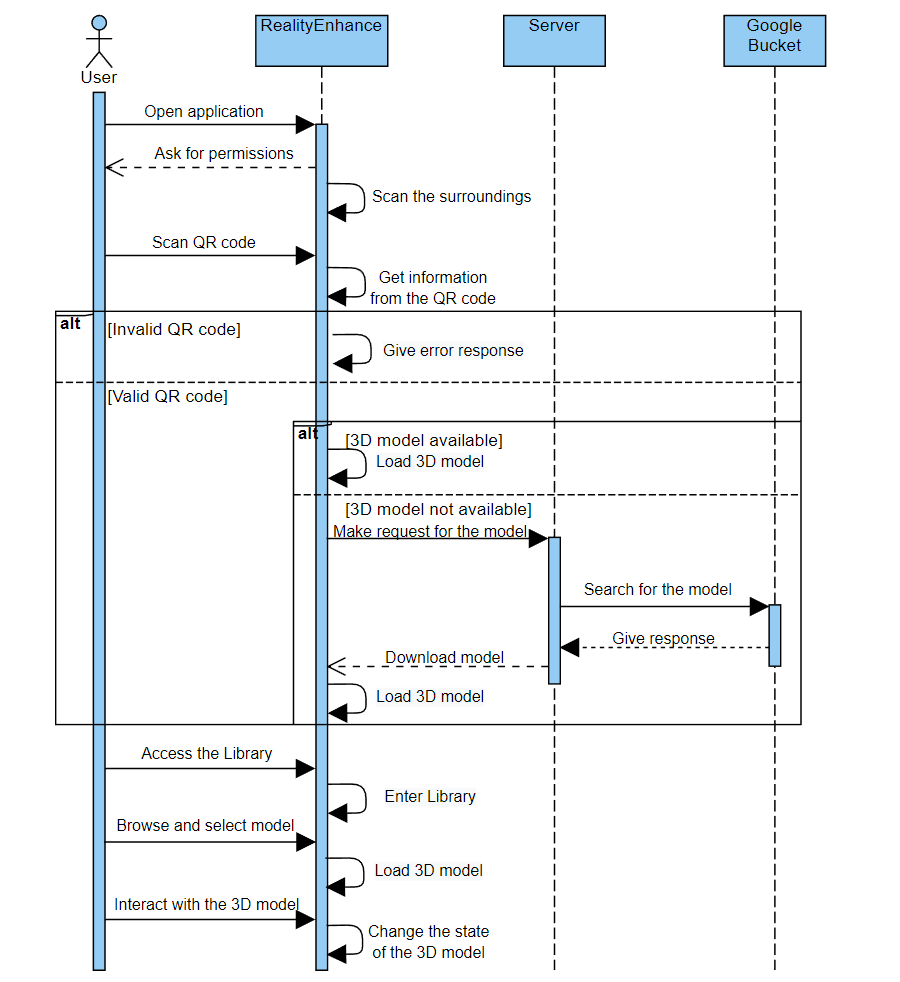
\includegraphics[width=1\textwidth]{img/SequenceDiagram.png}
    \caption{Sequence diagram}
    \label{fig:SequenceDiagram}
\end{figure}

\clearpage

\section{Implementation}
Implementation details...

\section{Deployment}
Deployment details...
